% Preamble
\documentclass[11pt]{article}
\usepackage{braket}
\usepackage{graphicx}
\usepackage[margin=1in]{geometry}

\usepackage{makeidx}  % allows for indexgeneration
\usepackage{ifpdf}
\usepackage{url}


\title{Elementary Cellular Automata as an Error Minimization Cryptographic Hash}
\date{November 2024}
\author{Daniel McKinley}

% Document
\begin{document}

\maketitle

\section{Introduction}

Elementary cellular automata (ECA) are 8 bit extensions of 4 bit logic gate truth tables, done linearly in parallel. \cite{Wolfram}
Here a subset of 8 of the 256 ECA rules are explored as a non-cryptographic hash function. It utilizes an error-minimization function on 4x4 binary grids; this parallels several discrete transforms, the Fast Fourier Transform (FFT) and Fast Walsh-Hadamard Transform. General algorithm, specific ECA rules, and aggregate properties are discussed. It is implemented in Java at \cite{mygit} along with more frames of the algorithm images. \\
\section{Main Algorithm}

\begin{center}
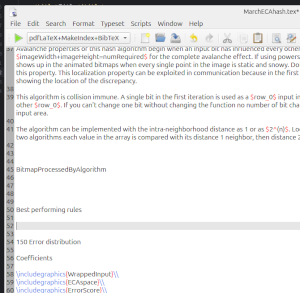
\includegraphics{testScreenshot}\\
Original Image\\
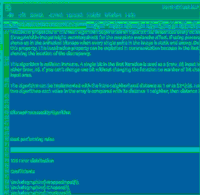
\includegraphics{processedDepth3}\\
Frame 3\\

\includegraphics{processedDepth6}\\
Frame 6\\
\end{center}

\begin{center}
There are $2^{16}=65536$ binary 4x4 arrays\\
 Where there are $2^4$ possible $row_0$ neighborhoods for a given ECA rule\\
 Each of these 16 input-ECAoutput arrays are scored by\\
\[  \sum_{r=0}^{3} \sum_{c=0}^{3} 2^r ( compressionAttempt_{r c} \oplus original_{r c}) \]\\
 The value of the neighborhoods of the minimum and maximum of these 16 sums are noted as the codeword pair of the original binary matrix  \\
\end{center}
The algorithm first creates a truth table for the lossy compression of square binary matrix using 1D ECA. For all $2^{16}=65536$ possibilities of a 4x4 binary array, wrap the columns so that the grid is cylindrical, use row 0 as the input neighborhood, of which there are $2^4=16$ possible. The remaining three rows for all 16 possible row 0 values is the ECA output on the cylinder. For the input row and three output rows, score the XOR difference between it and its binary 4x4 input. The errorScore for a codeword is the weighted sum of discrepancies between this codeword-produced output and the original 4x4 matrix Input[][], where the weight is a coefficient of $2^{row}$. The lowest and highest scoring neighborhoods out of the 16 calculated are then two hexadecimal codewords for the binary input neighborhood of size 4x4. All 65536 possible binary 4x4 matrices get a minimum and a maximum codeword.\\
\begin{center}
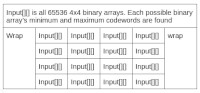
\includegraphics{inputGrid}\\
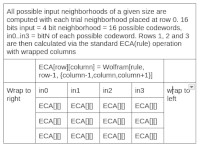
\includegraphics{ecaGrid}\\
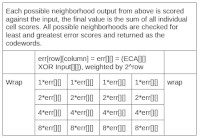
\includegraphics{errorGrid}\\
\end{center}

For every row,column location in input, that value's neighborhood is 4x4 (row,column)..((row+4),(column+4)). Every location is part of 16 neighborhoods. Transform the input so that each location is the minimizing and maximizing codewords of overlapping neighborhoods of the ECA rule subset described later.  Depths of iteration are the same process with the 4x4 neighborhoods' constituent rows and columns spaced out $2^{depth-1}$ instead of $2^{0}$. Depth 1 is next door neighboring codewords, depth 2 is two spaces away, depth 3 is 4 away. This comparing of neighbors of powers of 2 is the same arrow chart as the FFT and Fast Walsh Transform, except with reminimizations instead of sums and/or products at every level of recursion. These exponential neighborhood expansions guarantee the avalanche property in $log_2(size)$ time.\\
\begin{center}
Below is a Fast Walsh-Hadamard Example \cite{enwiki:1261916659}\\
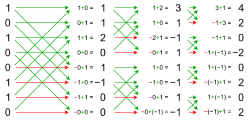
\includegraphics{FastWalshHadamard}\\
If you did the above with the powers of 2 in reverse order you would get this. Below is one axis of this algorithm, and instead of a sum term it's a sum term that gets reminimized. Find the codewords of the codewords, further apart each time.\\
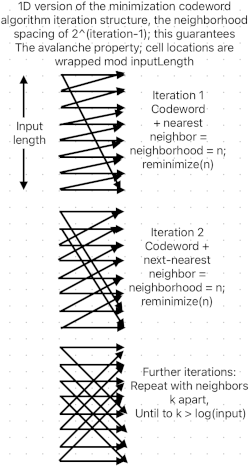
\includegraphics{AlgoStruct}\\
\end{center}

This transformation is 97\% invertible. A single rule of the positive 8-tuple of the below is a lossy compression algorithm with an error rate of 3/8. In a rectangular bitmap, the overlapping codeword, 16 4x4 neighbors that influence it, for all 8 of the rules in the subset together make a weighted vote on the inverse of the algorithm. 97 percent of bits were successfully recovered. Each codeword in the array produces a 4x4 ECA output that is its best guess about the information given to it. Each cell's 4x4 output overlaps with 4 of its neighbors. Each cell of each cell's output is weighted by its relative row and added to its location's tally of votes. At the end if the sum of the votes is positive then it becomes 0, if it is negative it becomes 1.\\

This algorithm both minimizes the errorScore in a lossy compression, and maximize the errorScore. There are dual min-max versions of most variables in the implementation.\\

\section{A subset of the 0-255 ECA}

There are 8 [0,15,51,85,170,204,240,255] of the 256 8 bit ECA truth tables that display the properties of unique codewords for any given input and perfectly even distribution of codewords. 0 and 255 are included because in the 4 rows of the output matrix, 1 is neighborhood input and 3 are output, and so still produce an errorScore and therefore a unique solution. This subset works with both errorScore minimization and errorScore maximization. This list shares most of its members with the XOR-additive list. \cite{xorAdditive} These two min max 8-tuples are implemented as sets of relevant Wolfram codes in the hash.\\

\section{Hash properties}

Codeword addition is each codeword's 4x4 ECA output is laid out flat like a piece of paper with another codeword, added, and then the combination is itself reminimized. In constructing the addition tables for codewords, the result was a table that is exactly the logical operation row AND column. The Hadamard matrix can be constructed using this operation by summing the ones in (row AND column) taking it mod 2 for the boolean Hadamard matrix. Experimentally, in the inverse phase the binary Hadamard value of the codeword was substituted for the codeword's 4x4 ECA output. The result had roughly the same 97\% decompression rate as the the first way. Each tuple rule's entire codeword output set was seperately processed as a weighted voting neighborhood without the overlap of the algorithm's main implementation. The result was 164/256 positively correlated Hadamard value to vote value. Each cell of each rule's Wolfram code does better than one half, then overlaps with 15 others al doing better than 1/2.\\

Avalanche properties of this hash algorithm begin when an input bit has influenced every other input bit. If using powers of two the avalanche effect begins at the greater of $log_2 (width) , log_2 (height)$. This property shows up in the animated bitmaps when every single point in the image is static and snowy. Doing fewer iterations than the avalanche's diffusion threshold but more than zero limits this property. This localization property can be exploited in communication because in the first few iterations the data is irreversible enough to be imperfectly unencryptable while showing the location of the discrepancy.\\

This algorithm has an optional loop that produces non-collisions. Without the optional loop collisions are experimentally noted as in the order of $1/10^14$. The non-collision loop takes the QR code Wolfram codes and each codeword becomes a 4x4 array of codewords of the wrap of the address. On their own codeword tuples are not distinct even if an individual tuple is; however this extra loop loops the codewords over themselves and the tuple becomes unique, eliminating the possibility of any collision. This extra wrap loop adds factor of 16 in both time and memory. Without that loop, random testing of collisions produced an one in a hundred trillion on a 5x5 matrix, random testing of larger arrays yielded none in any reasonable timeframe. Small scale local collisions are a possibility, large scale collisions are unlikely, and optionally no collisions.\\

The 8 Wolfram codes each have 256*256=65536 locations in the truth table. For each truth table, each codeword is used in 4096 locations. In terms of area, 1/256 pairs of locations share a codeword. So for 1 element of the 2 8-tuples collisions are common. When all 16 elements are bundled for a gridpoint in the bitmap input collisions are rare because 1/256 has to line up perfectly 6 times (some elements can be cancelled). When the optional loop is used the wrapping array eliminates any collisions.\\

What this transform is, intuitively, is hard to say at the moment. A Fourier transform flips the variable changes time to frequency. All the rules in the 8-tuple are of the form \{0,0,0,0,0,0,0,0\}, \{0,1,0,1,0,1,0,1\}, \{0,0,1,1,0,0,1,1\}, \{0,0,0,0,1,1,1,1\} as well as the complements. The first is a constant and the last three are not the XOR operation like 90 or 102, but the first half of the layers of an XOR table layered by place value. These rules can also be easily represented as a sin wave of frequencies in increments of $2^{-n}$. When an image is fully processed, each pixel's codeword set fully linearizes. 

\section{Bitmap Implementation}

The algorithm is prototyped on 4-byte RGB *.bmp bitmap files, including the first several images which come from a Linux screenshot then into *.bmp by GIMP. The program converts the image's raster in a rectangular hexadecimal matrix. Iteration 0 is the minimizing codewords for each location as is and then further iterations operate on neighboring hexadecimal codewords. Animated *.gif files are available at my website. You can see the areas of the image cloning itself 2 by 2 and slowly dissolving into avalanche territory that eventually just looks like noise everywhere. The current image was chosen because you can clearly see parts of the image doubling itself as the avalanche property slowly takes over. The code works with any size bitmap. Future work on the project would include other image formats as it is a color code hexadecimal conversion. 

\section{Other rules, shapes, and sizes}

The weight in the errorScore sum can be $2^{row}$ or $2^{column}$, both produce the same set of 8 tuples with the unique solution and even distribution properties, though other ECA rules' properties don't necessarily carry over. This transposition and reflections across an axis may be enough to produce unique tuples without the loop, however checking this is ongoing.\\

The size of the input array can be easily be any power of 2 squared. Calculation of Wolfram code lengths of $2^{16}$ are acceptable, lengths of $2^{64}$ would be challenging. At size 8 there are $2^8=256$ possible codewords that grow exponentially but not doubly exponentially because the codeword is only the first row of 8, which means that while you can't calculate the whole truth table at once you can calculate the codewords on the spot. The 8 tuple's uniqueness and distribution properties may or may not apply at size 8, it may not; it is only exhaustively tested for size 4.\\

Out of the other 0-255 ECA rules, some do better than these particular 8 at lossy compression, losing only 3/16 bits instead of 6/16 bits with these 8. In particular the Pascal rules 90, 165, 102, 153, 105, 150 rank near the top, connected to several these 8 via the property of XOR-additiveness (cite wolfram atlas). However none outside of these 8 have unique solutions or even distributions in either row or column weighted, maxxed or minned.\\

If while running this algorithm for rule 150 you produce a heat map of the errors in reconstructing the lossy compression, you get this. To seven binary digits, five past the decimal place, Phi and Pi show up in these ratios. Seven binary digits is a 2\% error rate. Seven digits is enough for an ASCII operation. Precision to seven decimal places shows up here and in reconstructing the 8-tuples above. If you label a five point star and proceed backwards starting at 0, you get \{3,1,4,2,0\} which is roughly the same seven digit precision. Some of those mentioned here are seven binary digits some are accurate to nine. While seven digits by itself is not impressive, 7 digits across three constants is notable.\\

\begin{center}
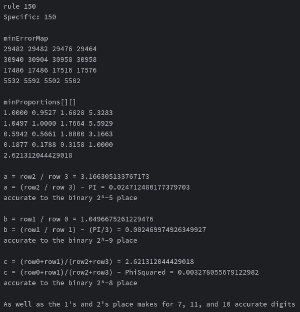
\includegraphics{PiRatios}\\
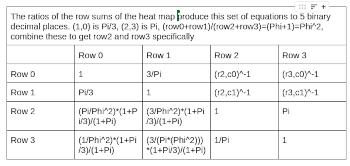
\includegraphics{RatioEquations}\\
\end{center}

\bibliographystyle{plain}
\bibliography{HashBib.bib}

\end{document}